\setmodule{9}

%BEGIN_FOLD % ====>>_____ Занятие 1 _____<<====
\begin{class}[number=1]
	\begin{listofex}
		\item Вычислите:
		\begin{tasks}(2)
			\task \( (\sqrt{13}-\sqrt{7})(\sqrt{13}+\sqrt{7}) \)
			\task \( \dfrac{ \sqrt{2,8} \cdot \sqrt{4,2} }{ \sqrt{0,24} } \)
			\task \( 7^{\tfrac{ 4 }{ 9 }} \cdot 49^{\tfrac{ 5 }{ 18 }} \)
			\task \( \dfrac{ 2^{3,5} \cdot 3^{5,5} }{ 6^{4,5} } \)
			\task \( \log_5 0,2 + \log_{0,5}4 \)
			\task \( \dfrac{ \log_3 25 }{ \log_3 5 } \)
		\end{tasks}
		%3
		\item
		\begin{minipage}[t]{0.45\linewidth}
			На рисунке изображен график функции \( y = f(x)\), определенной на интервале \((-5; 5)\). Найдите количество точек, в которых касательная к графику функции параллельна прямой \(y  =  6\) или совпадает с ней.
		\end{minipage}
		\hspace{0.02\linewidth}
		\begin{minipage}[t]{0.5\linewidth}
			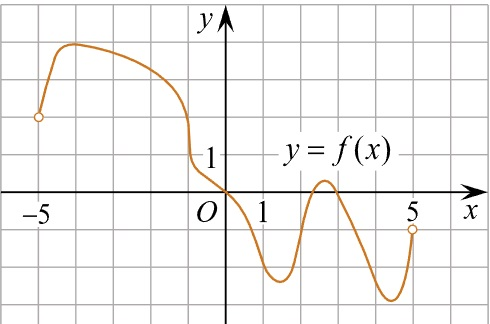
\includegraphics[align=t, width=\linewidth]{../\picpath/G111M5L2-1}
		\end{minipage}
		%4
		\item
		\begin{minipage}[t]{0.45\linewidth}
			На рисунке изображен график производной функции \(f(x)\), определенной на интервале \((-10; 2)\). Найдите количество точек, в которых касательная к графику функции \(f(x)\) параллельна прямой \(y = -2x - 11\) или совпадает с ней.
		\end{minipage}
		\hspace{0.02\linewidth}
		\begin{minipage}[t]{0.5\linewidth}
			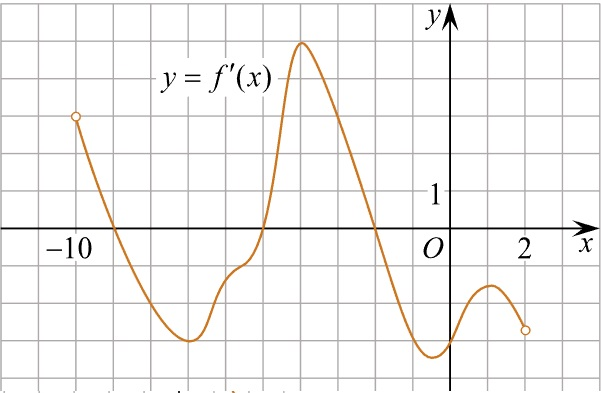
\includegraphics[align=t, width=\linewidth]{../\picpath/G111M5L2-2}
		\end{minipage}
		%5
		\item
		\begin{minipage}[t]{0.45\linewidth}
			На рисунке изображен график производной функции \(f(x)\), определенной на интервале \( (-6;6) \). Найдите промежутки возрастания функции \(f(x)\). В ответе укажите сумму целых точек, входящих в эти промежутки.
		\end{minipage}
		\hspace{0.02\linewidth}
		\begin{minipage}[t]{0.5\linewidth}
			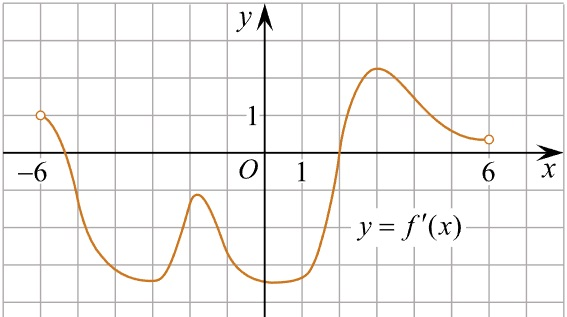
\includegraphics[align=t, width=\linewidth]{../\picpath/G111M5L2-3}
		\end{minipage}
		%6
		\item
		\begin{minipage}[t]{0.45\linewidth}
			На рисунке изображен график функции \(y = f(x)\), определенной на интервале \((-6; 8)\). Определите количество целых точек, в которых производная функции положительна.
		\end{minipage}
		\hspace{0.02\linewidth}
		\begin{minipage}[t]{0.5\linewidth}
			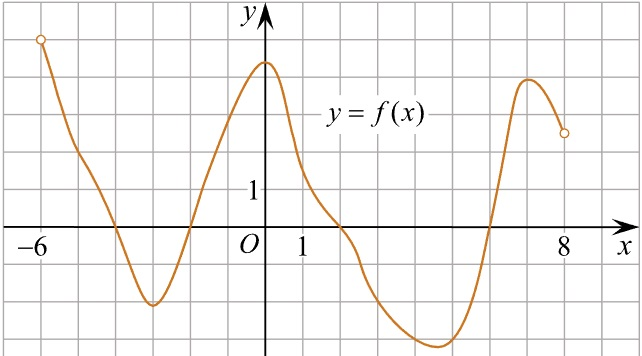
\includegraphics[align=t, width=\linewidth]{../\picpath/G111M5L2-4}
		\end{minipage}
		%7
		\item Найдите:
		\begin{tasks}(1)
			\task точку максимума функции \(y = 2x^3 -22x-15\)
			\task наименьшее значение функции \(y = 3x^3 - 54x\) на отрезке \([0;4]\)
			\task точку максимума функции \(y = x^3 - 5x^2 + 7x -5\)
			\task наименьшее значение функции \(y=(x-2)^2(x-4)+5\) на отрезке \( [1;3] \)
			\task наименьшее значение функции \(y=(x+3)^2(x+5)-1\) на отрезке \( [-4;-1] \)
			\task наибольшее точку минимума функции \(y=(x-2)^2(x-4)+5\)
			\task точку максимума функции \(y = -\dfrac{x^2+289}{x}\)
			\task наименьшее значение функции \(y = \dfrac{x^2+25}{x}\) на отрезке \([1;10]\)
			\task наименьшее точку максимума функции \(y=(x+16)e^{x-16}\)
			\task наименьшее точку минимума функции \(y=(9-x)e^{x+9}\)
			\task наименьшее значение функции \(y=4x-4\ln(x+7)+6\) на отрезке \( -6,5; 0 \)
			%\task наименьшее значение функции \( 12\cos x + 6 \sqrt{3}x-2\sqrt{3} + 0 \) на отрезке \( \left[ 0; \dfrac{ \pi }{ 2 } \right]  \)
			\task точку максимума функции \(y=\ln(x+5)^5-5x\)
			\task точку максимума функции \(y=3x-\ln(x+3)^3\)
			
			\task наименьшее значение функции \( (2x-3)\cos x - 2 \sin x + 5 \) на отрезке \( \left( 0; \dfrac{ \pi }{ 2 } \right) \)
			\task точку максимума функции \( y=(2x-3)\cos x - 2\sin x + 5 \), принадлежащую отрезку \( \left( 0;\dfrac{ \pi }{ 2 } \right) \)
			
		\end{tasks}
	\end{listofex}
\end{class}
%END_FOLD

%BEGIN_FOLD % ====>>_____ Занятие 2 _____<<====
\begin{class}[number=2]
	\begin{listofex}
		\item Занятие 2
	\end{listofex}
\end{class}
%END_FOLD

%BEGIN_FOLD % ====>>_ Домашняя работа 1 _<<====
\begin{homework}[number=1]
	\begin{listofex}
		\item Домашняя работа 1
	\end{listofex}
\end{homework}
%END_FOLD

%BEGIN_FOLD % ====>>_____ Занятие 3 _____<<====
\begin{class}[number=3]
	\begin{listofex}
		\item Занятие 3 
	\end{listofex}
\end{class}
%END_FOLD

%BEGIN_FOLD % ====>>_____ Занятие 4 _____<<====
\begin{class}[number=4]
	\begin{listofex}
		\item Занятие 4
	\end{listofex}
\end{class}
%END_FOLD

%BEGIN_FOLD % ====>>_ Домашняя работа 2 _<<====
\begin{homework}[number=2]
	\begin{listofex}
		\item Домашняя работа 2
	\end{listofex}
\end{homework}
%END_FOLD

%BEGIN_FOLD % ====>>_____ Занятие 5 _____<<====
\begin{class}[number=5]
	\begin{listofex}
		\item Занятие 5
	\end{listofex}
\end{class}
%END_FOLD

%BEGIN_FOLD % ====>>_____ Занятие 6 _____<<====
\begin{class}[number=6]
	\begin{listofex}
		\item Занятие 6
	\end{listofex}
\end{class}
%END_FOLD

%BEGIN_FOLD % ====>>_ Домашняя работа 3 _<<====
\begin{homework}[number=3]
	\begin{listofex}
		\item Домашняя работа 3
	\end{listofex}
\end{homework}
%END_FOLD

%BEGIN_FOLD % ====>>_____ Занятие 7 _____<<====
\begin{class}[number=7]
	\title{Подготовка к проверочной}
	\begin{listofex}
		\item Занятие 7
	\end{listofex}
\end{class}
%END_FOLD

%BEGIN_FOLD % ====>>_ Проверочная работа _<<====
\begin{exam}
	\begin{listofex}
		\item Проверочная
	\end{listofex}
\end{exam}
%END_FOLD